\subsubsubsubsection{Lane}
\begin{figure}[h]
\centering
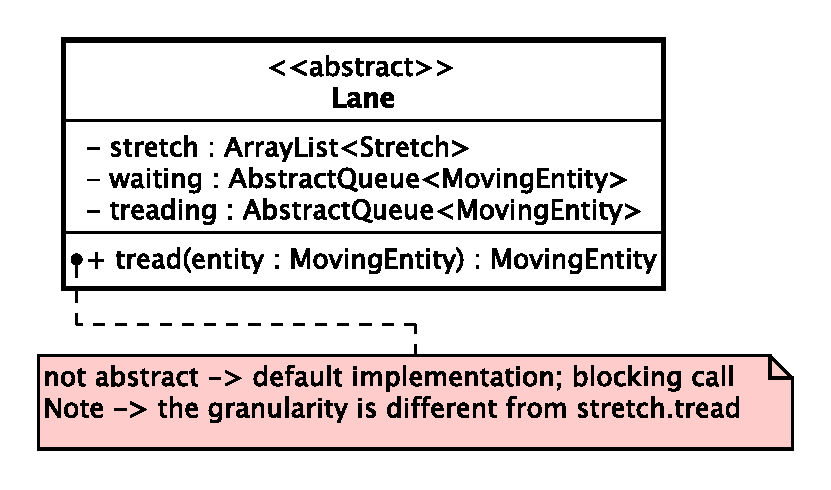
\includegraphics[scale=0.6,keepaspectratio]{images/solution/lane.eps}
\caption{App::Reactive::Lane}
\label{fig:sd-app-lane}
\end{figure}
\FloatBarrier
\begin{itemize}
  \item \textbf{Description} \\
    It represents a lane entity. It is a protected object composed of one or
    more stretches.
  \item \textbf{Attribute}
  \begin{itemize}
    \item \texttt{- size: Unsigned Int} \\
The size of the stretch/treading queue.
    \item \texttt{- stretch: ArrayList<Stretch>} \\
The list of stretches which compose the lane.
    \item \texttt{- treading: AbstractQueue<MovingEntity>} \\
The queue of moving entities which are treading the lane.
    \item \texttt{- waiting: AbstractQueue<MovingEntity>} \\
The queue of moving entities which are waiting to tread the lane. 
  \end{itemize}
  \item \textbf{Operation}
  \begin{itemize} 
    \item \texttt{+ Lane(size: Unsigned Int, stretch: ArrayList<Stretch>)} \\
Creates a \texttt{Lane} object with a specific size and list of stretches.
    \item \texttt{+ tread(entity: MovingEntity)} \\
Implements the lane treading. Moves the entity on the stretches which are 
in the moving entity route.
  \end{itemize}
\end{itemize}
